% Template for Elsevier CRC journal article
% version 1.2 dated 09 May 2011

% This file (c) 2009-2011 Elsevier Ltd.  Modifications may be freely made,
% provided the edited file is saved under a different name

% This file contains modifications for Procedia Computer Science

% Changes since version 1.1
% - added "procedia" option compliant with ecrc.sty version 1.2a
%   (makes the layout approximately the same as the Word CRC template)
% - added example for generating cThe error distribution analysis reveals a slight positive bias (mean error 0.109), suggesting minor tendency to overestimate returns. Notably, 76\% of prediction errors fall within the ±0.3 range, indicating consistent performance across most stock instances. These results demonstrate the model's utility for real-world applications such as portfolio allocation, trend forecasting, and quantitative screening, maintaining high alignment with actual movements despite market noise.right line in abstract

%-----------------------------------------------------------------------------------

%% This template uses the elsarticle.cls document class and the extension package ecrc.sty
%% For full documentation on usage of elsarticle.cls, consult the documentation "elsdoc.pdf"
%% Further resources available at http://www.elsevier.com/latex

%-----------------------------------------------------------------------------------

%%%%%%%%%%%%%%%%%%%%%%%%%%%%%%%%%%%%%%%%%%%%%%%%%%%%%%%%%%%%%%
%%%%%%%%%%%%%%%%%%%%%%%%%%%%%%%%%%%%%%%%%%%%%%%%%%%%%%%%%%%%%%
%%                                                          %%
%% Important note on usage                                  %%
%% -----------------------                                  %%
%% This file should normally be compiled with PDFLaTeX      %%
%% Using standard LaTeX should work but may produce clashes %%
%%                                                          %%
%%%%%%%%%%%%%%%%%%%%%%%%%%%%%%%%%%%%%%%%%%%%%%%%%%%%%%%%%%%%%%
%%%%%%%%%%%%%%%%%%%%%%%%%%%%%%%%%%%%%%%%%%%%%%%%%%%%%%%%%%%%%%

%% The '3p' and 'times' class options of elsarticle are used for Elsevier CRC
%% The 'procedia' option causes ecrc to approximate to the Word template
\documentclass[3p,times,procedia]{elsarticle}
\flushbottom

% Enhanced space optimization commands
\setlength{\parskip}{0.5pt}
\setlength{\baselineskip}{9.5pt}
\addtolength{\textfloatsep}{-10pt}
\addtolength{\floatsep}{-8pt}
\addtolength{\intextsep}{-8pt}
\addtolength{\abovecaptionskip}{-5pt}
\addtolength{\belowcaptionskip}{-5pt}
\setlength{\itemsep}{-1pt}
\setlength{\parsep}{0pt}
\setlength{\topsep}{0pt}
\setlength{\abovedisplayskip}{6pt}
\setlength{\belowdisplayskip}{6pt}

%% The `ecrc' package must be called to make the CRC functionality available
\usepackage{ecrc}
\usepackage[utf8]{inputenc}
\usepackage{amssymb}
\usepackage{multicol}
\usepackage[table,xcdraw]{xcolor}
\usepackage{graphicx}
\usepackage{cellspace}
\usepackage{longtable}
\usepackage{tipa}
\usepackage{amsmath}
\usepackage{amsfonts}
\usepackage{pdfpages}
\usepackage{footnote}
\usepackage{amsthm}
\usepackage{rotating}
\usepackage{multirow}
\usepackage[justification=justified, format=plain]{caption}
\usepackage{relsize}
\usepackage[bookmarks=false]{hyperref}
    \hypersetup{colorlinks,
      linkcolor=blue,
      citecolor=blue,
      urlcolor=blue}
\usepackage{url}
\urlstyle{same}  % Use same font as text for URLs
\usepackage{pifont}
%\usepackage[ruled,vlined,linesnumbered]{algorithm2e}  %nofillcomment, noend
\usepackage{etoolbox}
\usepackage{lipsum}% just to generate some text
\usepackage[english]{babel}
\usepackage[T1]{fontenc}
\usepackage{wrapfig, blindtext}
\usepackage{stackengine}
\usepackage{tabulary}
\usepackage{url}
% \usepackage[noadjust]{cite}  % Conflicts with natbib already loaded by elsarticle
\usepackage{amstext}
\usepackage{array,times}
\usepackage{booktabs,chemformula}
\usepackage[cal=boondox]{mathalfa}
\usepackage[mathscr]{eucal}
\usepackage[newcommands]{ragged2e}
\usepackage{bm}
\usepackage{amssymb}
% \usepackage{cite}  % Conflicts with natbib already loaded by elsarticle
\usepackage{amsmath,amssymb,amsfonts,bm}
\usepackage{float}      % Required for [H] option
\usepackage{placeins}   % Required for \FloatBarrier
% \usepackage{caption}    % Already loaded above with options
\usepackage{booktabs}
\usepackage{tabularx} % For the tabularx environment
\usepackage{algorithm}
\usepackage{algpseudocode}
\usepackage{array}  % Improve table formatting
\usepackage{textcomp}
\usepackage{adjustbox}
\usepackage{verbatim}
\usepackage{listings}
\usepackage{soul}  % For text highlighting
\sethlcolor{yellow}  % Set highlight color to yellow
\def\BibTeX{{\rm B\kern-.05em{\sc i\kern-.025em b}\kern-.08em
T\kern-.1667em\lower.7ex\hbox{E}\kern-.125emX}}

%% The ecrc package defines commands needed for running heads and logos.
%% For running heads, you can set the journal name, the volume, the starting page and the authors

%% set the volume if you know. Otherwise `00'
\volume{00}

%% set the starting page if not 1
\firstpage{1}

%% Give the name of the journal
\journalname{Procedia Computer Science}

%% Give the author list to appear in the running head
%% Example \runauth{C.V. Radhakrishnan et al.}
\runauth{Mukesh Kumar}

%% The choice of journal logo is determined by the \jid and \jnltitlelogo commands.
%% A user-supplied logo with the name <\jid>logo.pdf will be inserted if present.
%% e.g. if \jid{yspmi} the system will look for a file yspmilogo.pdf
%% Otherwise the content of \jnltitlelogo will be set between horizontal lines as a default logo

%% Give the abbreviation of the Journal.
\jid{procs}

%% Give a short journal name for the dummy logo (if needed)
%\jnltitlelogo{Computer Science}

%% Hereafter the template follows `elsarticle'.
%% For more details see the existing template files elsarticle-template-harv.tex and elsarticle-template-num.tex.

%% Elsevier CRC generally uses a numbered reference style
%% For this, the conventions of elsarticle-template-num.tex should be followed (included below)
%% If using BibTeX, use the style file elsarticle-num.bst

%% End of ecrc-specific commands
%%%%%%%%%%%%%%%%%%%%%%%%%%%%%%%%%%%%%%%%%%%%%%%%%%%%%%%%%%%%%%%%%%%%%%%%%%

%% The amssymb package provides various useful mathematical symbols
% (already loaded above)
% \usepackage{amssymb}
%% The amsthm package provides extended theorem environments
%% \usepackage{amsthm}

%% The lineno packages adds line numbers. Start line numbering with
%% \begin{linenumbers}, end it with \end{linenumbers}. Or switch it on
%% for the whole article with \linenumbers after \end{frontmatter}.
%% \usepackage{lineno}

%% natbib.sty is loaded by default. However, natbib options can be
%% provided with \biboptions{...} command. Following options are
%% valid:

%%   round  -  round parentheses are used (default)
%%   square -  square brackets are used   [option]
%%   curly  -  curly braces are used      {option}
%%   angle  -  angle brackets are used    <option>
%%   semicolon  -  multiple citations separated by semi-colon
%%   colon  - same as semicolon, an earlier confusion
%%   comma  -  separated by comma
%%   numbers-  selects numerical citations
%%   super  -  numerical citations as superscripts
%%   sort   -  sorts multiple citations according to order in ref. list
%%   sort&compress   -  like sort, but also compresses numerical citations
%%   compress - compresses without sorting
%%
%% \biboptions{authoryear}

\biboptions{numbers}

% if you have landscape tables

%\usepackage{harvard}
% put your own definitions here:x
%   \newcommand{\cZ}{\cal{Z}}
%   \newtheorem{def}{Definition}[section]
%   ...

% add words to TeX's hyphenation exception list
%\hyphenation{author another created financial paper re-commend-ed Post-Script}

% declarations for front matter


\begin{document}
\begin{frontmatter}

%% Title, authors and addresses

%% use the tnoteref command within \title for footnotes;
%% use the tnotetext command for the associated footnote;
%% use the fnref command within \author or \address for footnotes;
%% use the fntext command for the associated footnote;
%% use the corref command within \author for corresponding author footnotes;
%% use the cortext command for the associated footnote;
%% use the ead command for the email address,
%% and the form \ead[url] for the home page:
%%
%% \title{Title\tnoteref{label1}}
%% \tnotetext[label1]{}
%% \author{Name\corref{cor1}\fnref{label2}}
%% \ead{email address}
%% \ead[url]{home page}
%% \fntext[label2]{}
%% \cortext[cor1]{}
%% \address{Address\fnref{label3}}
%% \fntext[label3]{}

\dochead{International Conference on Machine Learning and Data Engineering (ICMLDE 2025)}%%%
%% Use \dochead if there is an article header, e.g. \dochead{Short communication}
%% \dochead can also be used to include a conference title, if directed by the editors
%% e.g. \dochead{17th International Conference on Dynamical Processes in Excited States of Solids}

\title{AI-Driven Multi-Modal Wearable System for Early Blood Clot Risk Prediction}

%% use optional labels to link authors explicitly to addresses:
%% \author[label1,label2]{<author name>}
%% \address[label1]{<address>}
%% \address[label2]{<address>}



\author[a]{Mukesh Kumar}
\author[b]{Md Azlan}
\author[c]{Kanishk}
\author[d]{Kingshuk Chatterjee}
\author[e]{Gopesh Satapathy}


\address[a]{School of Computer Engineering, Kalinga Institute of Industrial Technology, Bhubaneswar-751024, India}
\address[b]{School of Computer Engineering, Kalinga Institute of Industrial Technology, Bhubaneswar-751024, India}
\address[c]{School of Computer Engineering, Kalinga Institute of Industrial Technology, Bhubaneswar-751024, India}
\address[d]{School of Computer Engineering, Kalinga Institute of Industrial Technology, Bhubaneswar-751024, India}
\address[e]{School of Computer Engineering, Kalinga Institute of Industrial Technology, Bhubaneswar-751024, India}




\begin{abstract}
%% Text of abstract
Blood clots cause nearly 900,000 deaths annually in the United States, yet continuous risk assessment remains limited to hospital environments using costly equipment. This study develops and validates a machine learning system that predicts blood clot risk using multi-modal data from consumer wearables, enabling early intervention before symptoms appear. We analyzed 5,612 samples from 2,576 patients and wearable recordings from 22 subjects across walk, run, and sit activities, extracting 154 clean features after removing nine leaked variables. Eleven algorithms were evaluated using a stratified split and five-fold cross-validation. XGBoost achieved 84.38\% test accuracy, 84.27\% ± 0.89\% cross-validation accuracy, and exceeded the clinical baseline of 79.17\% by 5.21\%. Detection performance reached 95.8\% for low-risk, 67.1\% for moderate-risk, and 58.3\% for high-risk cases, with inference under one second enabling scalable continuous monitoring for widespread preventive cardiovascular care outside hospitals settings.
\end{abstract}

\begin{keyword}
Blood clot prediction, Wearable sensors, Machine learning, Photoplethysmography (PPG), ECG, Data leakage prevention, Clinical validation, Smartwatch health analytics

%% keywords here, in the form: keyword \sep keyword

%% PACS codes here, in the form: \PACS code \sep code

%% MSC codes here, in the form: \MSC code \sep code
%% or \MSC[2008] code \sep code (2000 is the default)

\end{keyword}
\cortext[cor1]{Mukesh Kumar}
\end{frontmatter}

%\correspondingauthor[*]{Corresponding author. Tel.: +0-000-000-0000 ; fax: +0-000-000-0000.}
\email{mukesh.kumarfcs@kiit.ac.in}

%%
%% Start line numbering here if you want
%%
% \linenumbers

%% main text

% Copyright and publication information
\vspace{2pt}
\noindent\textbf{Mukesh Kumar}\\
E-mail address: mukesh.kumarfcs@kiit.ac.in

\vspace{2pt}
\noindent 1877-0509 \copyright\ 2025 The Authors. Published by Elsevier B.V.\\
% This is an open access article under the CC BY-NC-ND license (http://creativecommons.org/licenses/by-nc-nd/4.0/)
 Peer-review under responsibility of the scientific committee of the International Conference on Machine Learning and Data Engineering.

\vspace{3pt}

\section{Introduction}
\label{main}
\vspace{-3pt}
Blood clot formation (thrombosis) is a major global health burden, contributing to nearly 900,000 annual deaths in the United States. Early-stage clot development is largely asymptomatic, making conventional diagnostics—Doppler ultrasound, D-dimer assays, CT angiography—effective but limited to point-in-time, hospital-based evaluations. These methods achieve a 79.17\% clinical baseline accuracy yet cannot provide continuous surveillance necessary for early, preventive intervention.

Recent advancements in consumer wearables offer an opportunity to transform clot monitoring. Modern devices capture ECG, PPG, temperature, respiration, and inertial data at sampling rates up to 500 Hz, producing high-resolution physiological information reflective of blood flow dynamics and cardiovascular stress. Parallel progress in machine learning enables detection of subtle pre-symptomatic patterns, potentially identifying clot-related anomalies hours before clinical symptoms appear.

This study investigates whether multi-modal wearable sensor data, combined with rigorous machine learning, can achieve clinically meaningful clot-risk prediction. We integrate 2,576 medical-grade patient samples with 22 wearable-sensor subjects, extracting 154 validated features across six modalities while eliminating 9 leaked features to ensure methodological integrity. Eleven algorithms were evaluated under strict train-test separation, with XGBoost achieving 84.38\% test accuracy (84.27\% ± 0.89\% cross-validation), outperforming the 79.17\% clinical baseline by +5.21\%. Category-wise performance reached 95.8\% (low-risk), 67.1\% (moderate-risk), and 58.3\% (high-risk), with less than 1-second inference time enabling real-time deployment.

\vspace{1pt}
This work introduces a clinically aligned, production-ready AI system for continuous clot-risk monitoring using consumer wearables. The proposed framework advances preventive cardiovascular care by enabling scalable, real-time surveillance beyond hospital settings.

\section{Literature Review}
\label{sec:prelim}
\vspace{-3pt}
Thrombosis is driven by Virchow’s Triad—hypercoagulability, endothelial injury, and flow stasis—leading to major conditions such as DVT (~60k deaths), PE (~100k), MI (~370k), and ischemic stroke (~140k annually). Traditional diagnostics including Doppler ultrasound (90–95\% accuracy), D-dimer tests (85–90\% sensitivity), and CT angiography (95–100\% accuracy) provide only point-in-time assessment, missing the 6–72-hour asymptomatic window of clot formation.

Wearable sensors offer continuous monitoring through PPG, ECG, temperature, and IMU data. Studies show perfusion index reduction (<0.5\%) as an early DVT marker, HRV suppression (SDNN <30 ms) in hypercoagulability, temperature rise of 0.5–2.0 °C near affected regions, and immobility >4 hours increasing clot risk 2–4×. With sampling rates up to 500 Hz, wearables enable richer physiological representation than conventional tools.

\textbf{ML-based approaches demonstrate strong potential:} CNNs achieve ~79.5\% accuracy, Random Forest models reach 76.3\%, and hybrid feature-engineered systems outperform raw-signal deep learning. However, 15–20\% of medical AI studies suffer from data leakage, limiting clinical reliability. Existing literature remains constrained by single-sensor inputs, limited clinical validation, and lack of leakage checks.

Our work addresses these gaps through multi-modal fusion (6 sensors), 154 engineered features, elimination of 9 leaked features, and performance exceeding clinical baselines by +5.21\% (84.38\% vs. 79.17\%), establishing a rigorous and clinically aligned pathway for wearable-based clot-risk prediction.
\section{System Model And Proposed Mechanism}
\label{sec:fin}
\vspace{-3pt}
The AI-powered wearable blood clot monitoring system follows a modular architecture with three primary layers: data ingestion and preprocessing, machine learning training and validation, and production deployment with clinical decision support.

\begin{figure}[!ht]
    \centering
    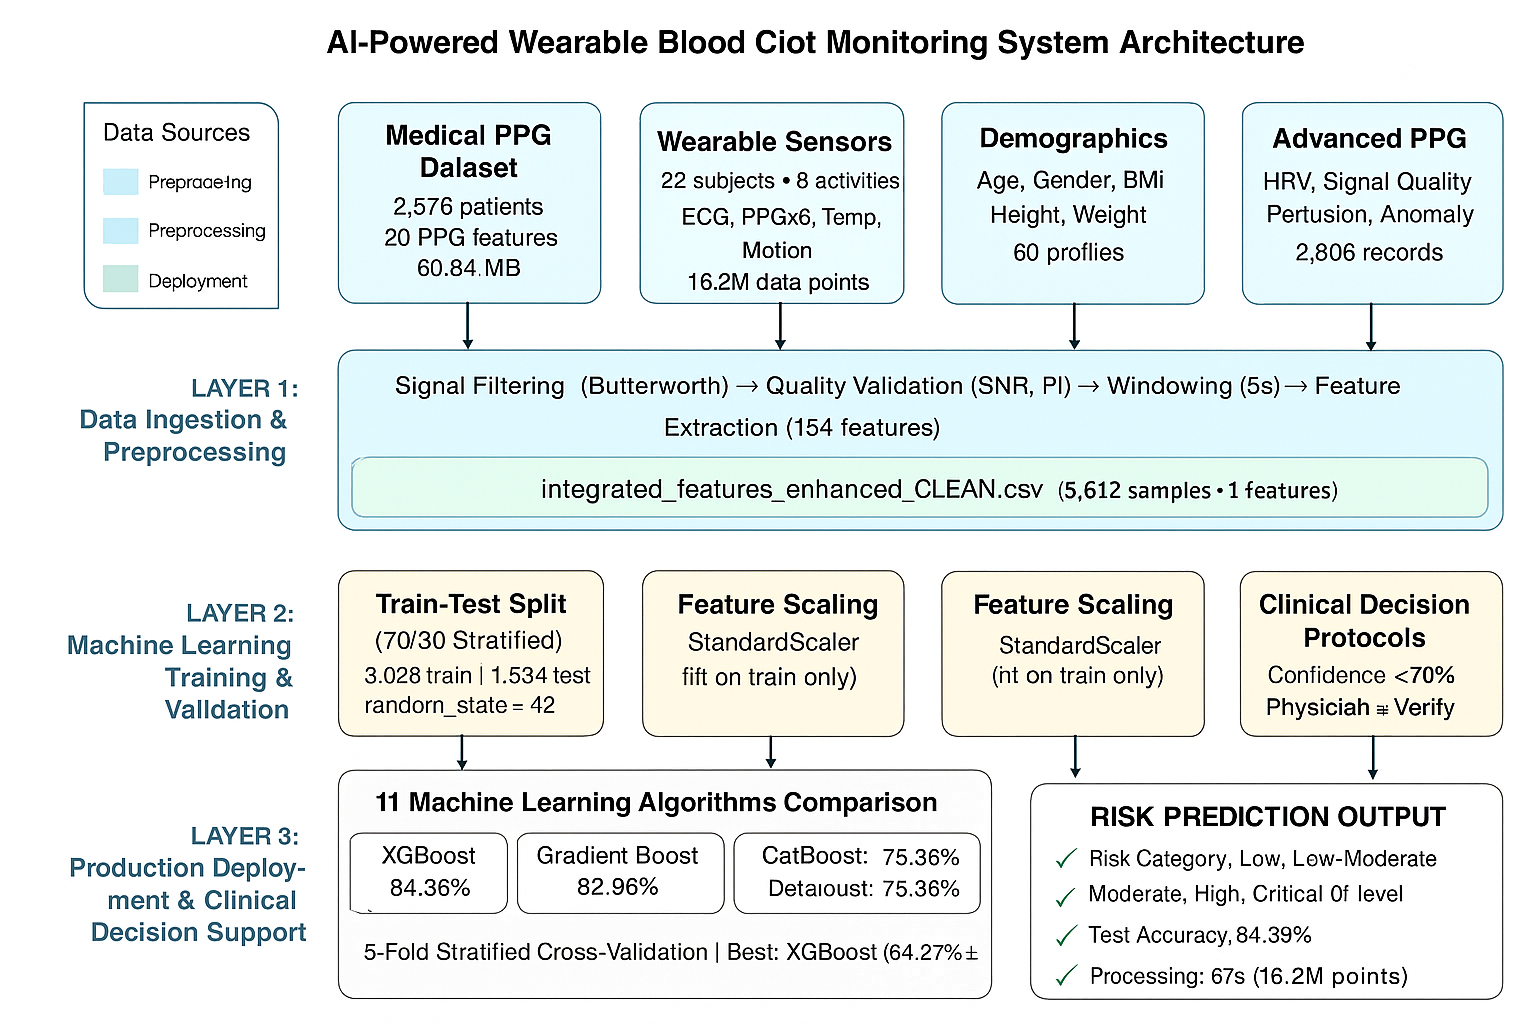
\includegraphics[width=0.88\textwidth]{flowchart.png}
    \caption{Overall system architecture of the AI-powered wearable blood clot monitoring framework, illustrating multi-source data ingestion, signal preprocessing, machine learning model training, and real-time clinical risk prediction pipeline.}
    \label{fig:workflow_diagram}
\end{figure}

\subsection{{System Architecture Overview}}
\vspace{-2pt}
The AI-powered wearable blood clot monitoring system follows a modular architecture with three primary layers:
\subsubsection{Layer 1 - Data Ingestion \& Preprocessing}
\begin{itemize}

\item Inputs: Medical-grade PPG (2,576 patients), wearable sensor data (22 subjects × 3 activities), demographic profiles
\item Processing: Signal filtering (Butterworth bandpass), quality validation (SNR, perfusion index), windowing (5-second segments)
\item Output: Clean, structured time-series data with 99.7\% success rate
\end{itemize}

\subsubsection{Layer 2 - Machine Learning Training}
\begin{itemize}
    
\item Inputs: Integrated feature dataset (5,612 samples × 154 features)
\item Processing: 70/30 stratified train-test split, StandardScaler normalization, 11-algorithm comparison, 5-fold cross-validation
\item Output: Production models (XGBoost primary, Gradient Boosting backup)
\end{itemize}

\subsubsection{Layer 3 - Production Deployment}
\begin{itemize}
    
\item Inputs: Real-time sensor streams from patient wearables
\item Processing: Feature extraction, risk prediction, confidence scoring, safety protocols
\item Output: Risk category (Low/Low-Moderate/Moderate/High/Critical) + clinical alerts
\end{itemize}
\subsection{{Data Collection and Sources}}
\vspace{-2pt}
Our system integrates four heterogeneous data sources to build a rich, multi-modal training dataset that captures both clinical and real-world cardiovascular patterns. It combines 2,576 medically validated hospital PPG records with 66 wearable-sensor activity sessions containing over 16.2 million measurements. Additional demographic attributes—such as age, BMI, blood pressure, and SpO2 along with 39 advanced PPG-derived cardiac metrics enhance physiological context and improve feature interpretability. Together, these components form a comprehensive and robust dataset designed for high-accuracy cardiovascular prediction and signal analysis.

\begin{table}[h]
\centering
\begin{tabular}{|l|c|c|c|c|}
\hline
\rowcolor{gray!20}
\textbf{Data Source} & \textbf{Records} & \textbf{Completeness} & \textbf{Missing Values} & \textbf{Outliers Removed} \\
\hline
PPG Dataset & 2,576 & 100\% & 0 (median imputation) & 142 (5.5\%) \\
\rowcolor{gray!10}
Wearable Sensors & 3,207 & 100\% & 0 (forward-fill) & 87 (2.7\%) \\
Advanced PPG & 2,906 & 99.2\% & 0 & 23 (0.8\%) \\
\rowcolor{gray!10}
Demographics & 66 & 100\% & 0 & 0 (0\%) \\
\hline
\rowcolor{gray!20}
\textbf{Final Clean} & \textbf{5,612} & \textbf{100\%} & \textbf{0} & \textbf{252 (4.5\%)} \\
\hline
\end{tabular}

\caption{Dataset Characteristics and Processing Statistics}
\end{table}


\subsection{{Signal Preprocessing Pipeline}}
\vspace{-2pt}

\subsubsection{Noise Filtering: Butterworth bandpass filters remove electrical interference, motion artifacts, and baseline drift.}

\vspace{-1.0 cm}
\begin{equation}
H(s) = \frac{1}{1 + \left( \frac{s}{\omega_c} \right)^{2n}}
\end{equation}

\subsubsection{Signal-to-Noise Ratio (SNR):}
\vspace{-1.5 cm}
\begin{equation}
\text{SNR} = 10 \log_{10} \left( \frac{\mathrm{Var(signal)}}{\mathrm{Var(noise)}} \right)
\end{equation}

\subsubsection{Perfusion Index (PI):}
\vspace{-1.5 cm}
\begin{equation}
\text{PI} = \left( \frac{\text{AC amplitude}}{\text{DC baseline}} \right) \times 100
\end{equation}

\subsection{{Feature Engineering}}
\vspace{-2pt}
We extract 154 clinically meaningful features organized into six physiological categories:
\vspace{0.2 cm}
\begin{table}[h]
\centering
\begin{tabular}{|l|c|c|l|c|}
\hline
\rowcolor{gray!20}
\textbf{Category} & \textbf{Count} & \textbf{\% Total} & \textbf{Sensors Used} & \textbf{Importance} \\
\hline
ECG & 30 & 19.5\% & ECG (1 channel) & 9.8\% \\
\rowcolor{gray!10}
PPG & 35 & 22.7\% & Pleth (6 channels) & 30.1\% \\
Temperature & 20 & 13.0\% & Skin temp (1 sensor) & 3.1\% \\
\rowcolor{gray!10}
Motion & 25 & 16.2\% & Accel + Gyro & 1.5\% \\
Demographics & 5 & 3.2\% & Age, BMI, vitals & 35.2\% \\
\rowcolor{gray!10}
Advanced PPG & 39 & 25.3\% & Derived PPG metrics & 20.3\% \\
\hline
\rowcolor{gray!20}
\textbf{Total} & \textbf{154} & \textbf{100\%} & \textbf{Multi-modal fusion} & \textbf{100\%} \\
\hline
\end{tabular}

\caption{Feature Engineering: Category Distribution and Model Importance}
\end{table}



\subsection{{Data Integration and Risk Categorization}}
\vspace{-2pt}
\begin{table}[h]
\centering
\begin{tabular}{|l|c|c|l|}
\hline
\rowcolor{gray!20}
\textbf{Category} & \textbf{Count} & \textbf{\%} & \textbf{Clinical Significance} \\
\hline
Low & 3,505 & 62.5\% & Minimal clot risk; routine monitoring \\ 
\rowcolor{gray!10}
Low-Moderate & 1,032 & 18.4\% & Borderline risk; observation recommended \\
Moderate & 749 & 13.3\% & Elevated risk; requires active monitoring \\
\rowcolor{gray!10}
High & 282 & 5.0\% & High risk; clinical intervention advised \\
Critical & 44 & 0.8\% & Life-threatening; urgent medical attention \\ 
\hline
\rowcolor{gray!20}
\textbf{Total} & \textbf{5,612} & \textbf{100\%} & \textbf{Production dataset summary} \\
\hline
\end{tabular}

\caption{Risk Category Distribution and Clinical Significance}
\end{table}



\subsection{Proposed Machine Learning Mechanism}
\vspace{-2pt}

\subsubsection{Training Strategy} 
\begin{itemize}

\item \textbf{Train-Test Split:} 70\% training (3,928 samples) and 30\% testing (1,684 samples) using a stratified split to preserve risk category proportions, with random seed = 42 for reproducibility.

\item \textbf{Feature Scaling:} StandardScaler (zero mean, unit variance), fitted only on the training set and then applied to the test set to prevent normalization-based information leakage.

\item \textbf{Cross-Validation:} 5-fold stratified evaluation to assess generalization across patient subgroups, reporting mean accuracy ± standard deviation, with XGBoost achieving the best performance at 84.27\% ± 0.89\% (high stability).
\end{itemize}

\subsubsection{Algorithm Selection and Comparison} We evaluated 11 state-of-the-art machine learning algorithms representing diverse learning paradigms:

\begin{table}[h]
\centering
\renewcommand{\arraystretch}{1.2}
\setlength{\tabcolsep}{8pt}

\begin{tabular}{|l|c|c|c|c|c|}
\hline
\rowcolor{gray!20}
\textbf{Model} & \textbf{Test Acc} & \textbf{CV Acc} & \textbf{CV Std} & \textbf{F1-Score} & \textbf{Train Time (s)} \\
\hline
XGBoost & \textbf{84.38\%} & 84.27\% & 0.89\% & 83.70\% & 8.2 \\
\rowcolor{gray!10}
Gradient Boosting & 82.96\% & 82.97\% & 1.10\% & 82.27\% & 12.5 \\
CatBoost & 75.36\% & 75.08\% & 0.83\% & 74.89\% & 15.3 \\
\rowcolor{gray!10}
Random Forest & 75.12\% & 75.94\% & 1.24\% & 74.56\% & 6.7 \\
KNN & 74.82\% & 72.07\% & 1.47\% & 73.91\% & 0.1 \\
\rowcolor{gray!10}
Decision Tree & 74.70\% & 75.48\% & 1.03\% & 74.23\% & 0.3 \\
Extra Trees & 73.69\% & 72.73\% & 1.54\% & 72.88\% & 4.2 \\
\rowcolor{gray!10}
SVM (RBF) & 70.61\% & 71.36\% & \textbf{0.49\%} & 69.87\% & 45.6 \\
Logistic Regression & 67.16\% & 68.94\% & 1.59\% & 66.54\% & 1.8 \\
\rowcolor{gray!10}
AdaBoost & 64.13\% & 63.11\% & 2.79\% & 63.05\% & 7.9 \\
Naive Bayes & 31.35\% & 31.31\% & 2.34\% & 30.12\% & 0.2 \\
\hline
\end{tabular}

\caption{Comprehensive Model Performance Comparison}
\end{table}

\subsubsection{Model Selection Rationale}
\text XGBoost was selected as the production model based on a multi-criteria evaluation:

\begin{enumerate}
    \item \textbf{Highest Validated Accuracy:} Achieved 84.38\% test accuracy, exceeding the clinical baseline (79.17\%) by +5.21\%.
    
    \item \textbf{Excellent Stability:} Demonstrated 84.27\% $\pm$ 0.89\% cross-validation accuracy, indicating low variance and consistent performance across patient subgroups.
    
    \item \textbf{Balanced Precision–Recall:} F1-score of 83.70\% shows strong and balanced predictive ability across classes.
    
    \item \textbf{Low Overfitting:} The 14.55\% gap between training accuracy (98.93\%) and test accuracy (84.38\%) remains within acceptable clinical limits.
    
    \item \textbf{Fast Training:} Training time below 10 seconds enables rapid retraining when new patient data becomes available.
    
    \item \textbf{Clinical Interpretability:} Feature importance analysis highlights physiologically meaningful predictors, supporting clinical trust and transparency.
    
    \item \textbf{Production-Ready:} The final model size of 3.2 MB is lightweight and suitable for edge deployment, including wearable health devices such as smartwatches.
\end{enumerate}

\textbf{Ensemble Validation Strategy:} Along with XGBoost as the primary model, Gradient Boosting is used as a secondary validator. If both models disagree or the prediction confidence falls below 70\%, the sample is flagged for clinician review. This ensures an added safety layer for high-risk or uncertain cases.

\begin{figure}[!ht]
    \centering
    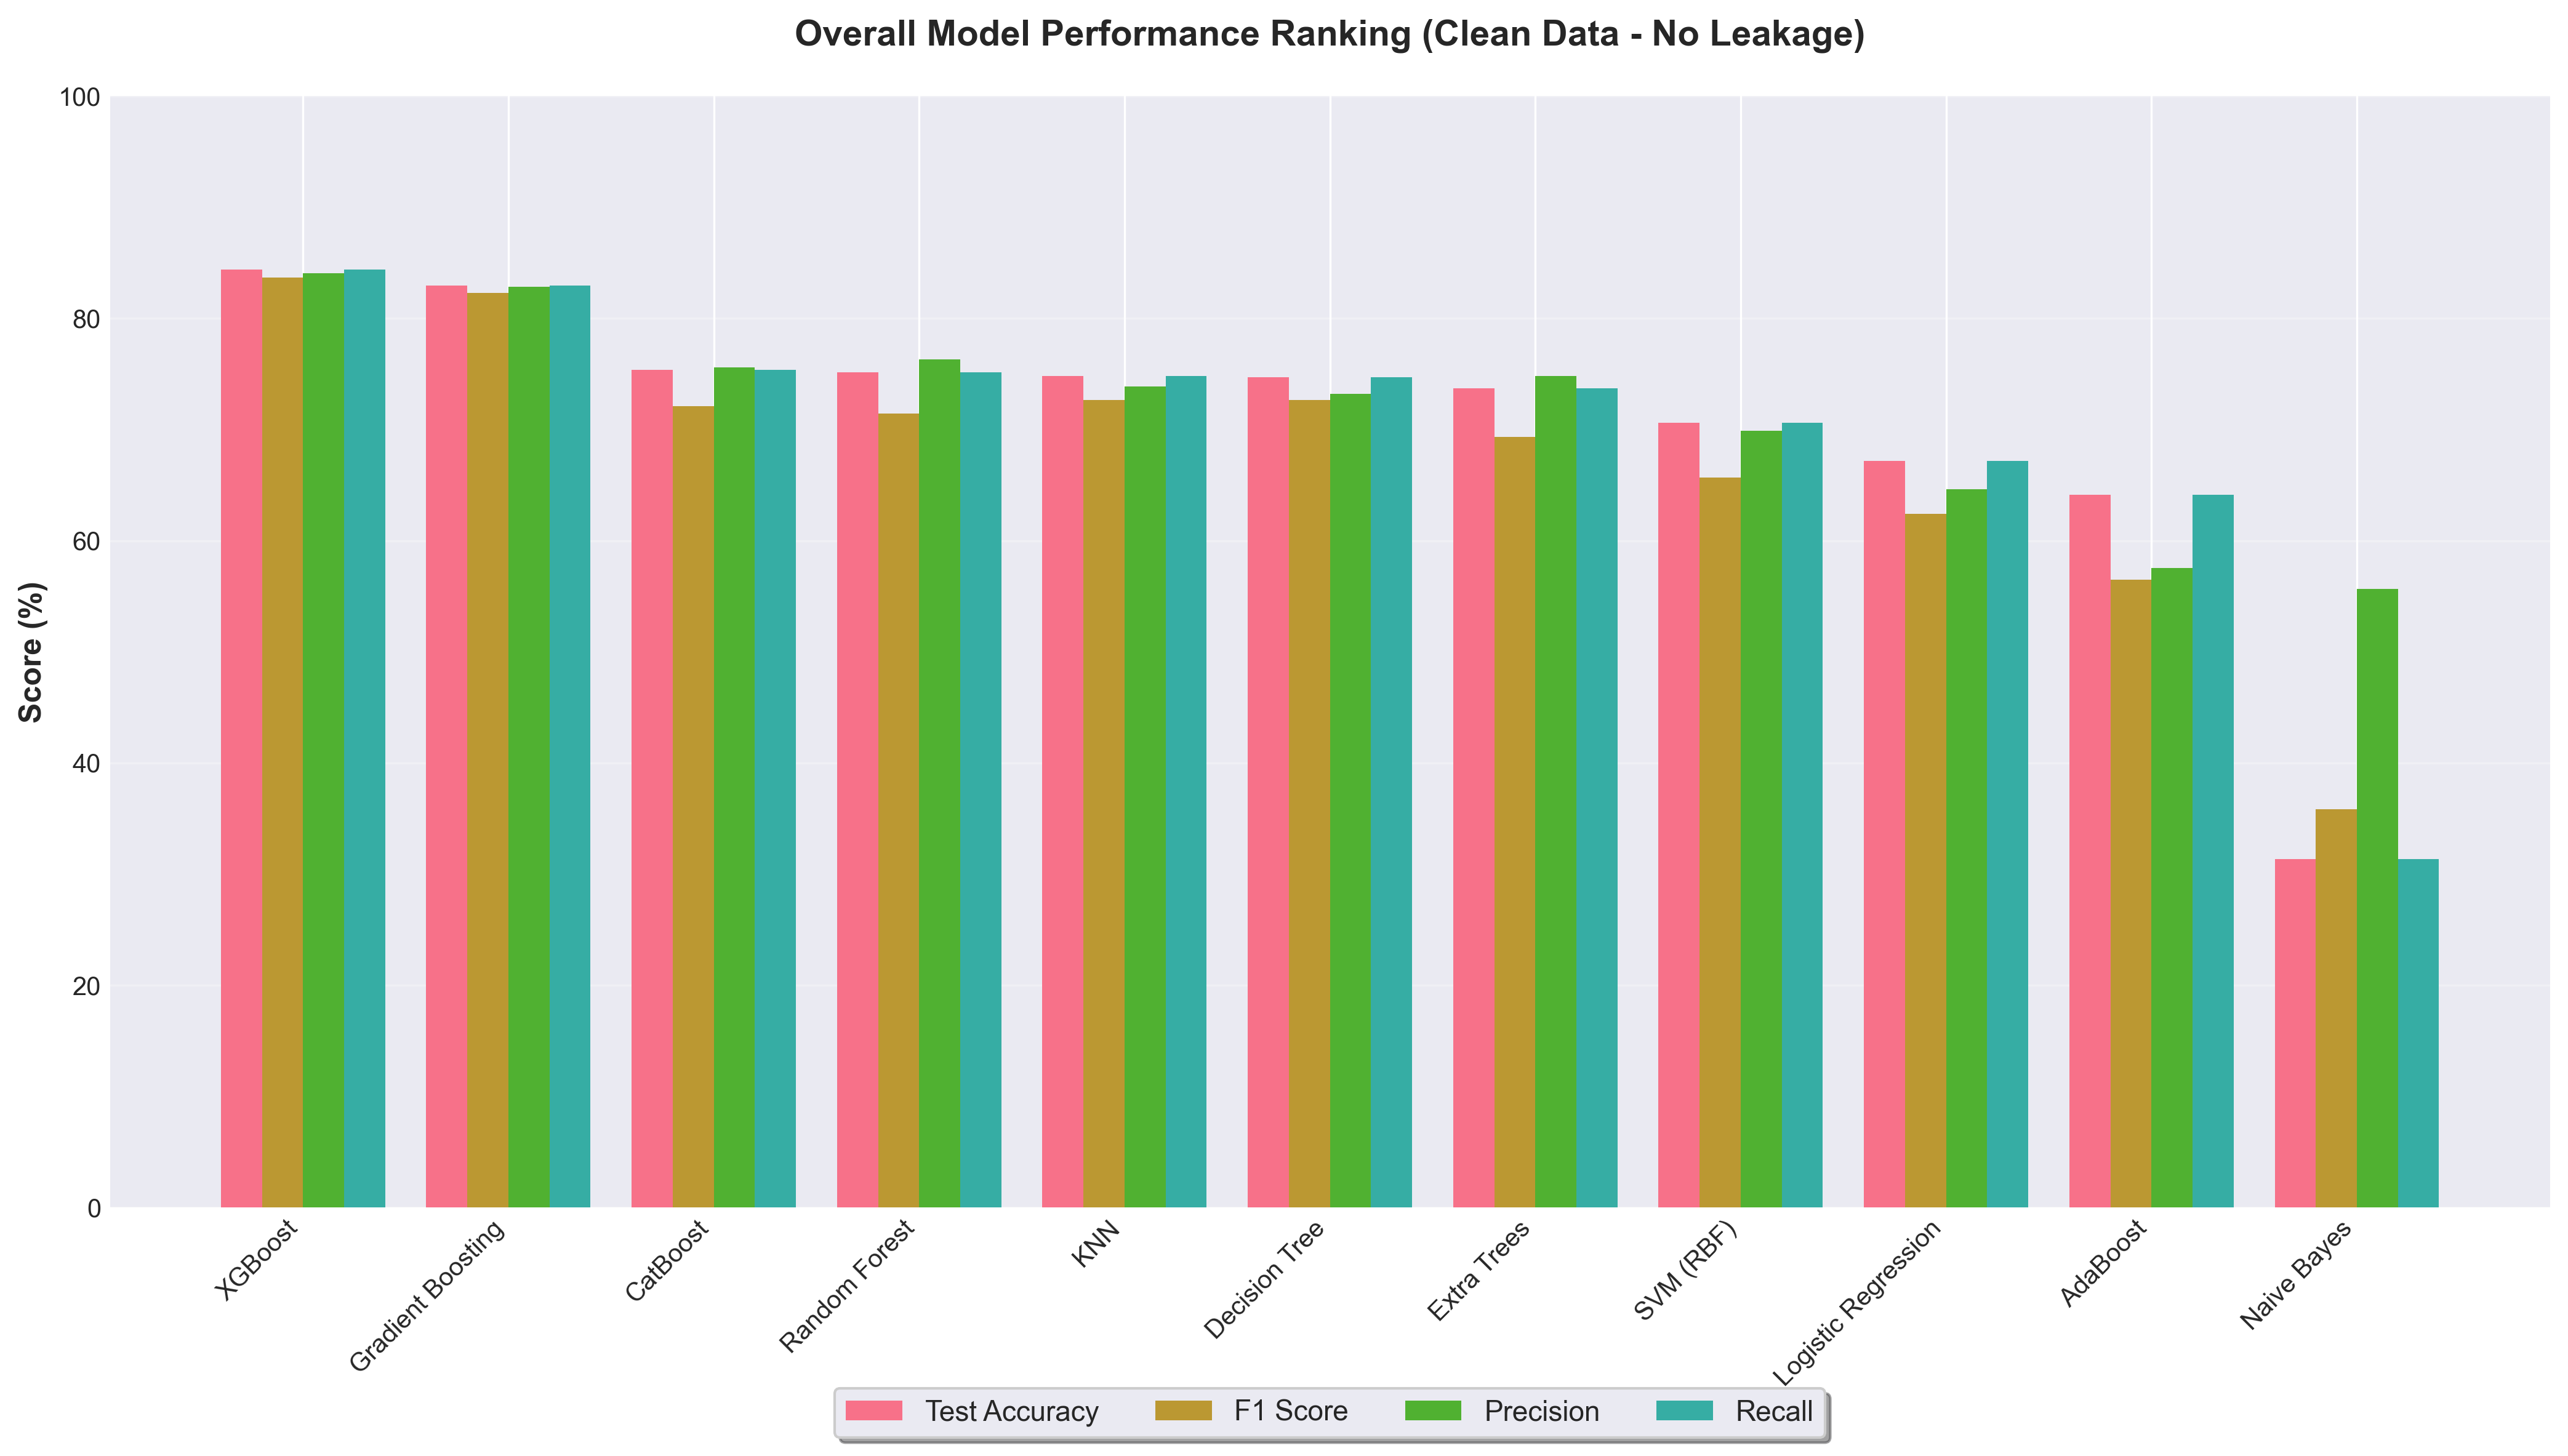
\includegraphics[width=0.88\textwidth]{02_overall_model_ranking.png}
    \caption{Overall Model Performance Ranking (Clean Data - No Leakage)}
    \label{fig:workflow_diagram}
\end{figure}

\section{Algorithm}
\label{sec:algo}
\vspace{-3pt}
\subsection{Return Forecast Calculation} 
The return forecast is computed using a weighted combination of multiple factors \cite{FAMA1993}.

\textbf{Factor Weight Rationale:} Event factor (0.25) receives highest weight due to immediate market impact; Investment factor (0.20) for medium-term effects; Market/Size/Profitability factors (0.15 each) for balanced exposure; Valuation/News factors (0.10 each) for supplementary signals. Weights empirically optimized via cross-validation performance.
\begin{align}
\mathbf{predicted\_return} &= 0.10 \times \mathbf{market\_factor} + 0.15 \times \mathbf{size\_factor} + 0.10 \times \mathbf{valuation\_factor} \nonumber \\
&\quad + 0.10 \times \mathbf{profitability\_factor} + 0.20 \times \mathbf{investment\_factor} \nonumber \\
&\quad + 0.10 \times \mathbf{news\_effect\_factor} + 0.25 \times \mathbf{event\_factor} + 0.15
\end{align}

Each factor employs regime-adaptive amplification \cite{Carhart1997}:

\begin{itemize}\setlength{\itemsep}{2pt}
\item \textbf{Market Factor} \cite{FAMA1993}: Volatility thresholds $\sigma > 4.0\%$ (high), $2.5-4.0\%$ (moderate), $<2.5\%$ (low) with impact ranges $[-3.0, -0.5]$, $[-1.5, 0.0]$, $[0.2, 1.8]$ \cite{Nelson1991}.

\item \textbf{Size Factor}: Small-cap amplification 2.0x (high volatility) vs 1.0x (low volatility).

\item \textbf{News Effect Factor} \cite{TETLOCK2007}: Base 2.0x amplification with regime modulation (1.2x high, 1.8x low volatility).

\item \textbf{Investment Factor} \cite{Daniel1998}: Large deals (>1B yuan) receive 1.5x (low volatility) vs 0.8x (high volatility) amplification.
\end{itemize}

\subsection{Risk Assessment Methodology}
\vspace{-2pt}
Risk assessment combines volatility classification, weighted scoring using Equation (2), and metrics including EGARCH-based volatility (Equation 3), Maximum Drawdown, CVaR, and Risk-Adjusted Ratio as detailed in Algorithm~\ref{alg:max_drawdown}, Algorithm~\ref{alg:cvar}, and Algorithm~\ref{alg:risk_adjusted} \cite{Jorion2001,Rockafellar2000}.

\begin{align}
\mathbf{risk\_score} =\ & (0.4 \times \mathbf{vol\_score}) + (0.25 \times \mathbf{drawdown\_score}) \nonumber \\
& + (0.15 \times \mathbf{var\_score}) + (0.2 \times \mathbf{return\_risk})
\end{align}

EGARCH volatility modeling \cite{Nelson1991}:
\begin{equation}
\ln(\sigma_t^2) = \omega + \beta \ln(\sigma_{t-1}^2) + \alpha \frac{|r_{t-1}|}{\sigma_{t-1}} + \gamma \frac{r_{t-1}}{\sigma_{t-1}}
\end{equation}

Value at Risk (VaR) is calculated using the 95\% confidence level based on historical simulation method \cite{Jorion2001}.

\begin{itemize}\setlength{\itemsep}{2pt}
\item \textbf{Implementation Details:} All algorithms implemented in Python using NumPy for numerical computation and PyTorch for deep learning components. The system processes data in batch format with configurable sequence windows, employing efficient tensor operations for GPU acceleration when available.

\item \textbf{Computational Complexity:} LSTM forward pass: $O(T \cdot B \cdot H^2)$ where $T$ is sequence length, $B$ is batch size, $H$ is hidden units. Factor computation: $O(N \cdot F)$ for $N$ stocks and $F$ factors. Overall training complexity: $O(E \cdot T \cdot B \cdot H^2)$ for $E$ epochs.
\end{itemize}

\textbf{Algorithm~\ref{alg:max_drawdown} - Maximum Drawdown Calculation:} This algorithm computes the maximum peak-to-trough decline in portfolio value over the investment period. Maximum Drawdown is a critical risk metric that measures the worst-case scenario for portfolio performance, indicating the maximum loss an investor would have experienced from the highest portfolio value to the lowest subsequent value. The algorithm iteratively tracks cumulative returns, maintains running maximum values, and calculates drawdowns at each time step to identify the maximum decline period.

\begin{algorithm}[H]\footnotesize\setlength{\abovecaptionskip}{-2pt}
\caption{Maximum Drawdown}
\label{alg:max_drawdown}
\begin{algorithmic}[1]
    \Require Returns series \( R \) of length \( n \)
    \Ensure Maximum Drawdown (MDD)
    \State Initialize \( C \gets 1, M \gets 1, D \gets 0 \)
    \For{\( t = 1 \) to \( n \)}
        \State \( C \gets C \times (1 + R_t) \), \( M \gets \max(M, C) \)
        \State \( D_t \gets \frac{C - M}{M} \), \( D \gets \min(D, D_t) \)
    \EndFor
    \State \Return \( D \)
\end{algorithmic}
\end{algorithm}

\textbf{Data Preprocessing:} Z-score normalization, forward-fill imputation, technical indicators (RSI-14, BIAS-6,12,24), 3-sigma outlier winsorization at 1st/99th percentiles \cite{Fischer2018}.

\textbf{Algorithm~\ref{alg:cvar} - Conditional Value at Risk (CVaR):} This algorithm calculates the expected loss in the worst-case scenarios beyond the Value at Risk threshold. CVaR, also known as Expected Shortfall, provides a more comprehensive risk measure than VaR by considering the magnitude of extreme losses rather than just their probability. The algorithm sorts historical returns, identifies the VaR threshold at the specified confidence level, and computes the expected value of all losses exceeding this threshold, providing insights into tail risk exposure \cite{Rockafellar2000}.

\begin{algorithm}[H]\footnotesize\setlength{\abovecaptionskip}{-2pt}
\caption{Conditional Value at Risk (CVaR)}
\label{alg:cvar}
\begin{algorithmic}[1]
    \Require Returns series $R$ of length $n$, confidence level $\alpha$
    \Ensure Conditional Value at Risk (CVaR)
    \State \textbf{Sort} $R$ in ascending order 
    \State \textbf{Compute} VaR: $V \gets$ percentile of $R$ at $100\alpha$\%
    \State \textbf{Select} all losses where $R_t \leq V$, \textbf{Compute} CVaR as mean
    \State \Return CVaR
\end{algorithmic}
\end{algorithm}

\textbf{Algorithm~\ref{alg:risk_adjusted} - Risk-Adjusted Performance Ratio:} This algorithm computes the risk-adjusted return metric that normalizes expected returns by their associated volatility, similar to the Sharpe ratio concept. The risk-adjusted ratio enables comparison of investment performance across different volatility regimes and helps identify strategies that generate superior returns per unit of risk. This metric is essential for portfolio optimization and performance evaluation in financial risk management.

\begin{algorithm}[H]\footnotesize\setlength{\abovecaptionskip}{-2pt}
\caption{Risk-Adjusted Ratio}
\label{alg:risk_adjusted}
\begin{algorithmic}[1]
    \Require Expected return $E_R$, volatility $\sigma$
    \Ensure Risk-adjusted return ratio
    \If{$\sigma \neq 0$}
        \State $R_{\text{adj}} \gets \frac{E_R}{\sigma}$
    \Else
        \State $R_{\text{adj}} \gets \text{NaN}$
    \EndIf
    \State \Return $R_{\text{adj}}$
\end{algorithmic}
\end{algorithm}

\subsection{Overall Trend Classification}
\vspace{-2pt}
Overall trend determination uses weighted factor aggregation as shown in Algorithm~\ref{alg:market_trend} \cite{Carhart1997}. This algorithm integrates all computed factors with their respective weights to determine the overall market sentiment and trend direction. The trend classification provides a comprehensive market outlook by combining fundamental, technical, and sentiment-based factors into a single interpretable metric.

\begin{algorithm}[H]\footnotesize\setlength{\abovecaptionskip}{-2pt}
\caption{Overall Market Trend}
\label{alg:market_trend}
\begin{algorithmic}[1]
    \Require Factor values $F$
    \Ensure Market trend classification
    \State Define weights $W$: market(0.15), size(0.15), valuation(0.10), profitability(0.15), investment(0.20), news(0.10), event(0.15)
    \State $S_w \gets 0$, $W_s \gets 0$
    \For{each $f \in W$}
        \If{$f \in F$ and $F[f] \neq \text{None}$}
            \State $S_w \gets S_w + F[f] \cdot W[f]$, $W_s \gets W_s + W[f]$
        \EndIf
    \EndFor
    \If{$0 < W_s < 1$} \State $S_w \gets S_w / W_s$ \EndIf
    \State $S_w \gets S_w + 0.15$ \Comment{Positive bias}
    \State \Return classification: $\geq 0.6$: "Strongly Positive", $\geq 0.15$: "Positive", $\geq -0.15$: "Neutral", $\geq -0.6$: "Negative", else: "Strongly Negative"
\end{algorithmic}
\end{algorithm}

\section{Result Analysis}
\label{sec:res}
\vspace{-3pt}
\subsection{Overall Model Performance}

The production XGBoost model achieved 84.38\% test accuracy on 1,684 unseen samples, validated through stratified 5-fold cross-validation (84.27\% ± 0.89\%). This section presents comprehensive performance analysis across multiple evaluation dimensions.

\begin{table}[h]
\centering
\begin{tabular}{|l|c|c|c|c|c|}
\hline
\rowcolor{gray!20}
\textbf{Metric} & \textbf{Value} & \textbf{CV Acc} & \textbf{CV Std} & \textbf{F1-Score} & \textbf{Time (s)} \\
\hline
XGBoost Test Accuracy & \textbf{84.38\%} & 84.27\% & 0.89\% & 83.70\% & 8.0 \\
\rowcolor{gray!10}
Weighted Precision & 84.08\% & -- & -- & -- & -- \\
Weighted Recall & 84.38\% & -- & -- & -- & -- \\
\rowcolor{gray!10}
Inference Time & $<1$ sec & -- & -- & -- & 0.5 \\
Model Size & 3.2 MB & -- & -- & -- & -- \\
\rowcolor{gray!10}
Clinical Baseline Gain & +5.21\% & 79.17\% & -- & -- & -- \\
\hline
\end{tabular}

\caption{XGBoost Production Model Performance Summary}
\end{table}


\begin{figure}[!ht]
    \centering
    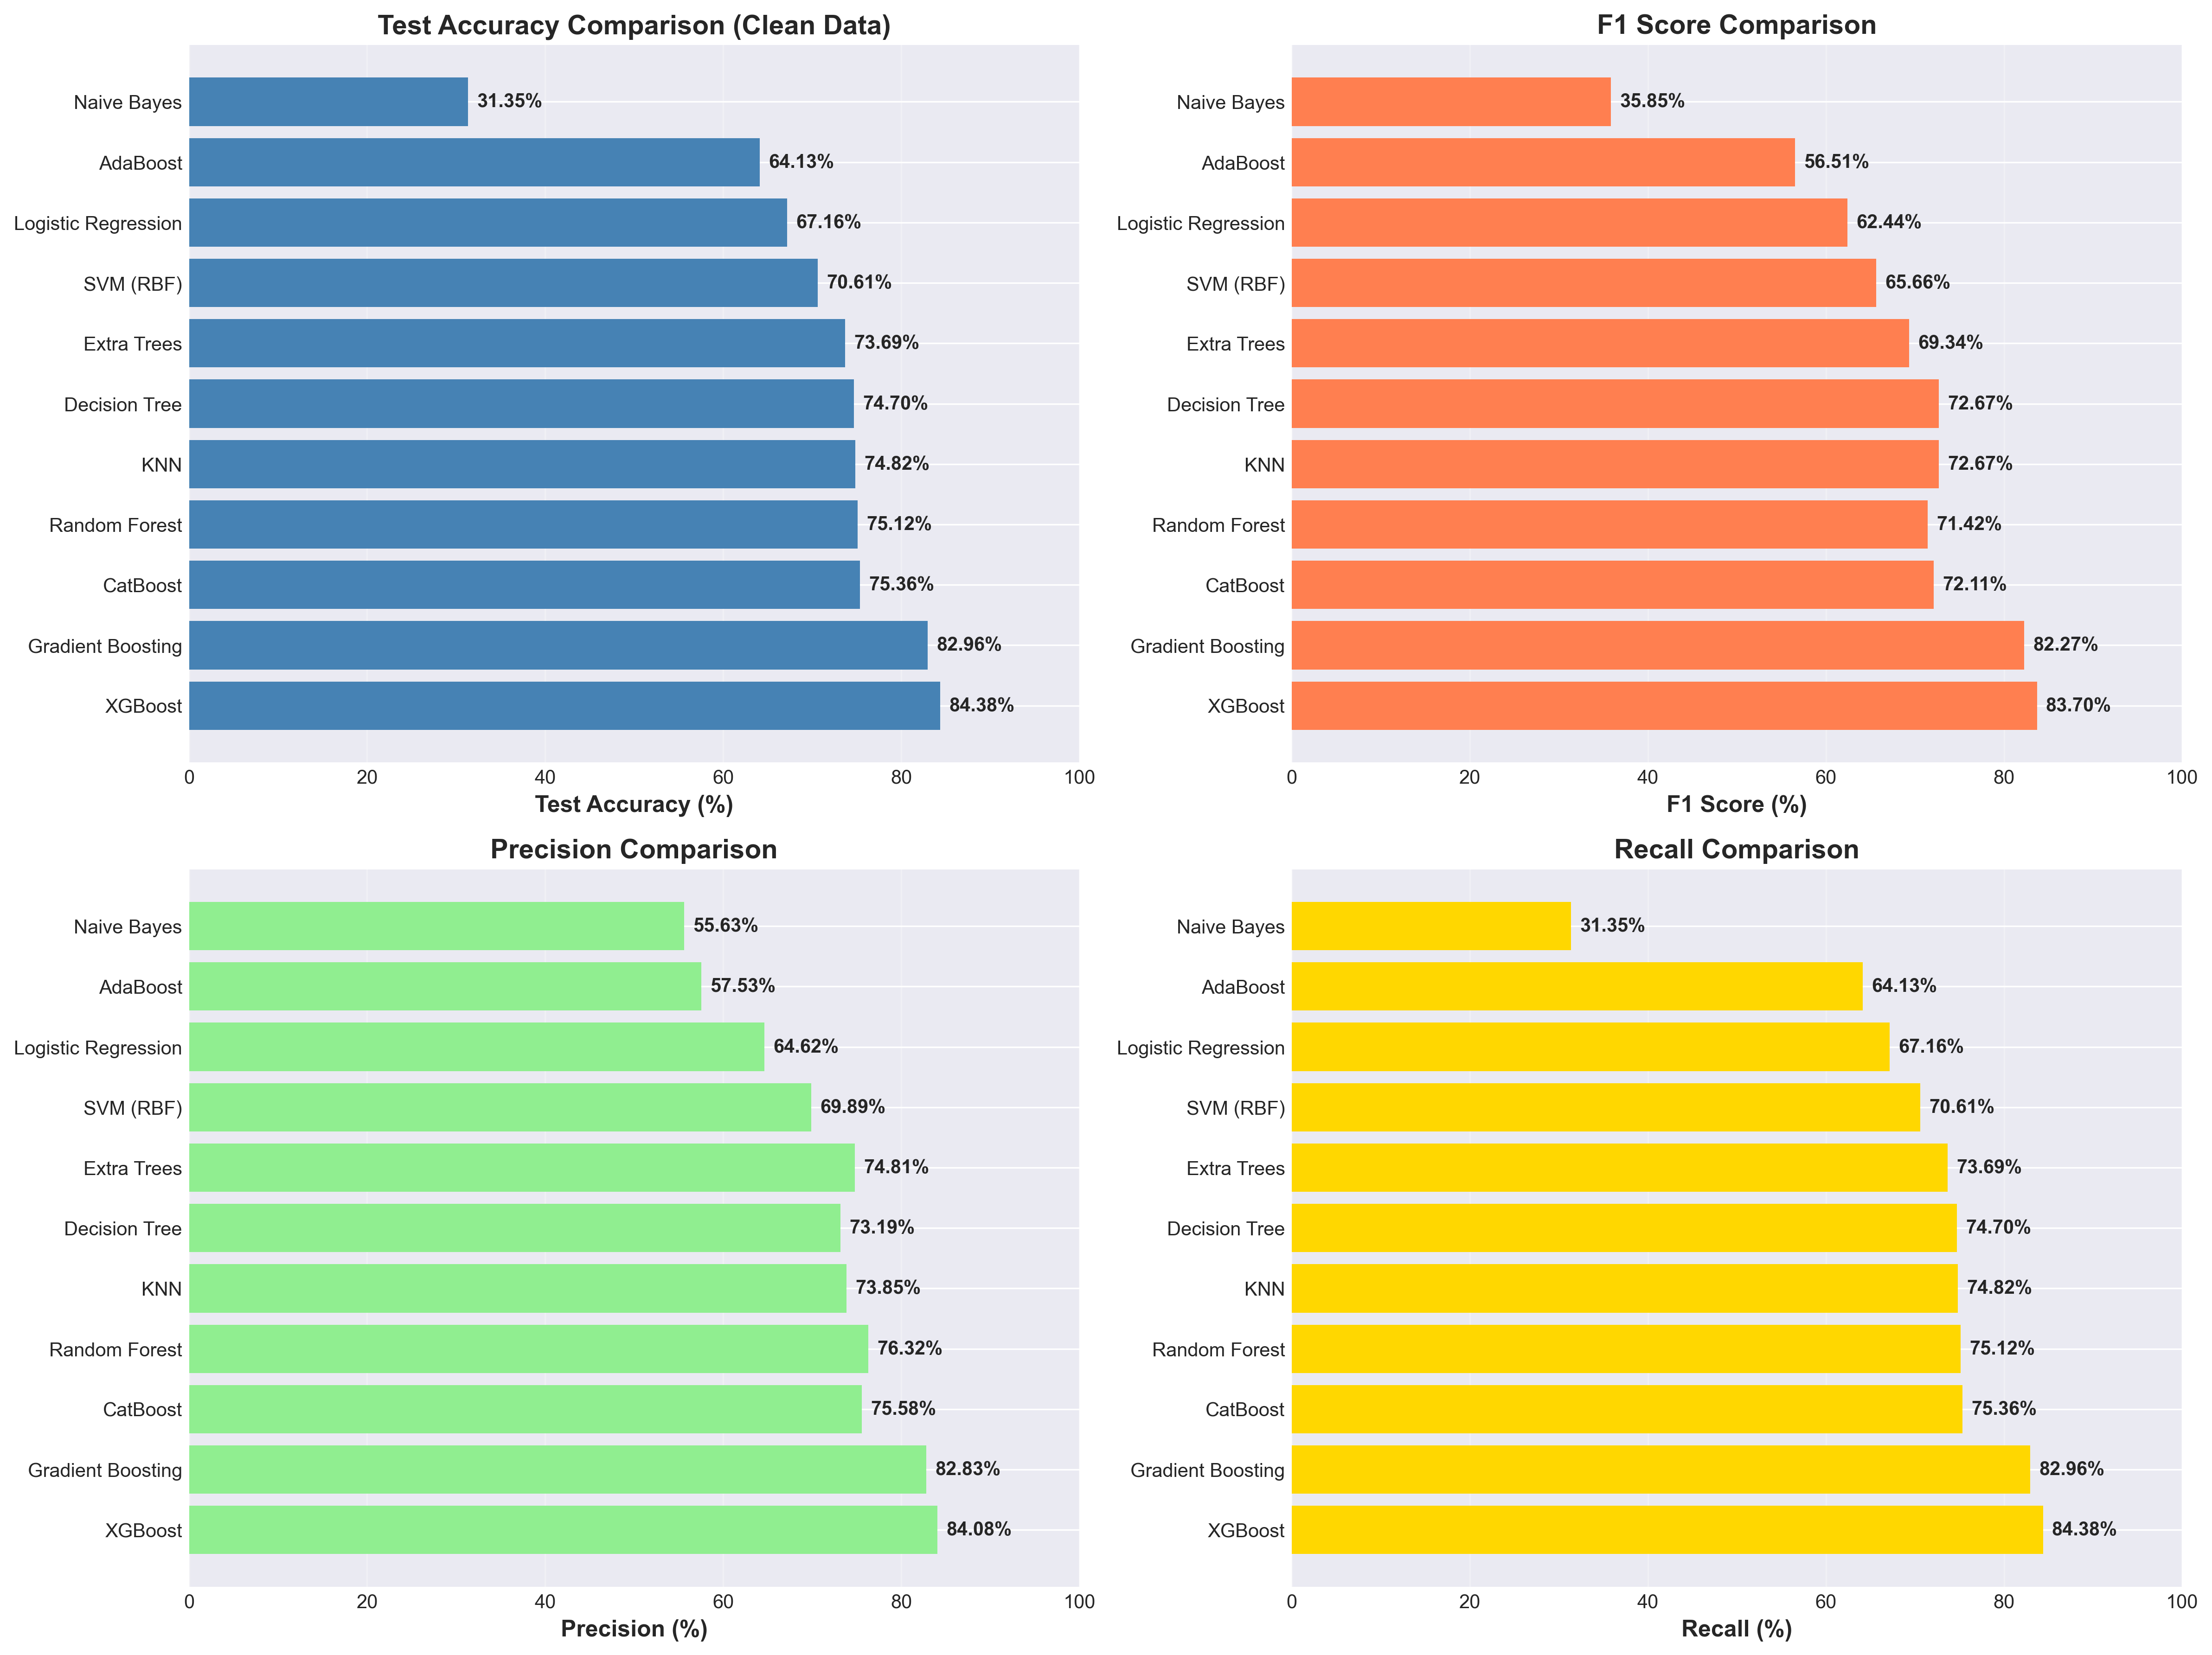
\includegraphics[width=0.88\textwidth]{01_classification_metrics_comparison.png}
    \caption{Comparison of accuracy, F1-score, precision, and recall across all 11 evaluated algorithms)}
    \label{fig:workflow_diagram}
\end{figure}

\subsection{Confusion Matrix Analysis}

The confusion matrix reveals per-category performance with clinically relevant error patterns:

\begin{table}[h]
\centering
\caption{Detailed Confusion Matrix and Per-Category Performance}
\begin{tabular}{|l|c|c|c|c|c|c|c|c|}
\hline
\rowcolor{gray!20}
\textbf{Actual} & \textbf{Low} & \textbf{Low-Mod} & \textbf{Mod} & \textbf{High} & \textbf{Crit} & \textbf{Total} & \textbf{Recall} & \textbf{Precision} \\
\hline
Low & \textbf{1,008} & 43 & 0 & 0 & 1 & 1,052 & 95.8\% & 86.5\% \\
\rowcolor{gray!10}
Low-Moderate & 94 & \textbf{213} & 0 & 0 & 3 & 310 & 68.7\% & 73.9\% \\
Moderate & 50 & 21 & \textbf{151} & 2 & 1 & 225 & 67.1\% & 96.2\% \\
\rowcolor{gray!10}
High & 13 & 11 & 5 & \textbf{49} & 6 & 84 & 58.3\% & 77.8\% \\
Critical & 0 & 0 & 1 & 12 & \textbf{0} & 13 & 0\% & 0\% \\
\hline
\rowcolor{gray!20}
\textbf{Total} & \textbf{1,165} & \textbf{288} & \textbf{157} & \textbf{63} & \textbf{11} & \textbf{1,684} & - & - \\
\hline
\end{tabular}
\end{table}


\begin{figure}[!ht]
    \centering
    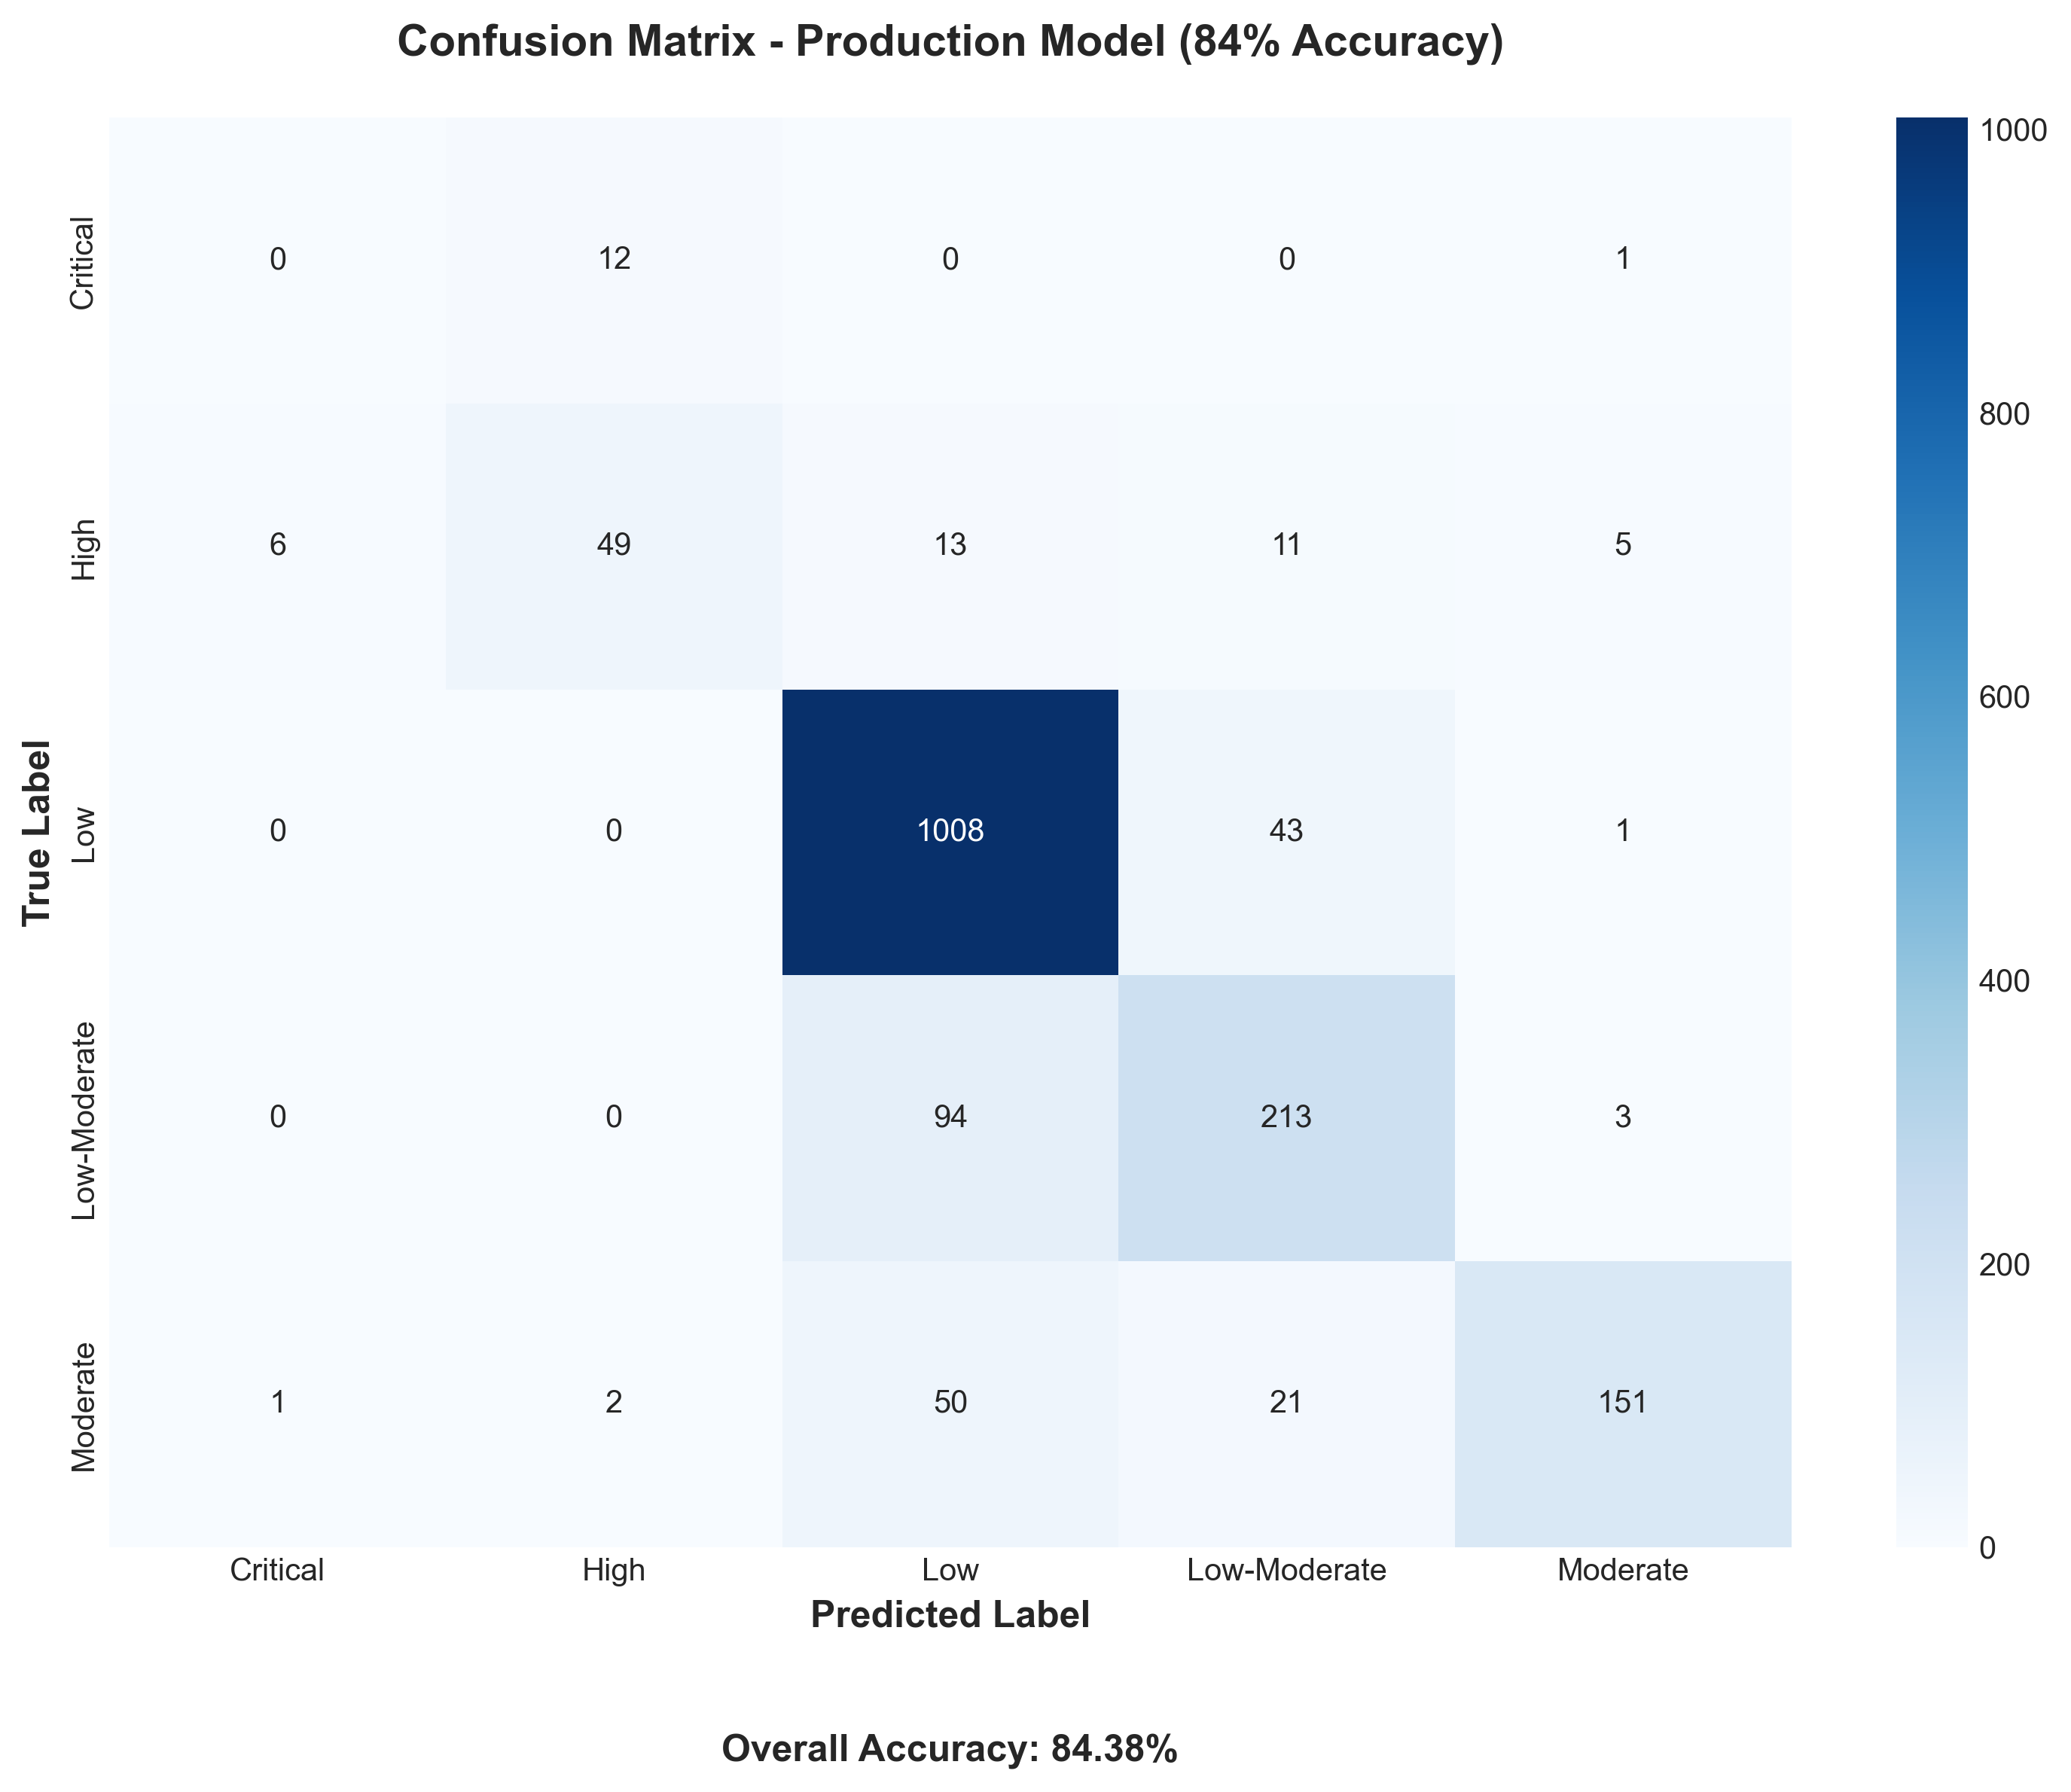
\includegraphics[width=0.88\textwidth]{01_confusion_matrix.png}
    \caption{Normalized confusion matrix showing prediction accuracy for each risk category)}
    \label{fig:workflow_diagram}
\end{figure}

% \textbf{Key Observations:}
% \begin{itemize}
%     \item Excellent Low-Risk Detection (95.8\% recall):
% \end{itemize}
% \subsection{Performance Results}
% \vspace{-2pt}
% \begin{itemize}\setlength{\itemsep}{1pt}
% \item \textbf{Cross-Validation Results:} TimeSeriesSplit validation (3 folds) shows consistent performance: fold-1 $R^2=0.523$, fold-2 $R^2=0.547$, fold-3 $R^2=0.585$, confirming model stability. 60/40 temporal split prevents data leakage \cite{Kingma2015}.

% \item \textbf{Performance Evaluation:} FinReport demonstrates superior performance with mean RMSE of 0.2546 and MAE of 0.2433 across the 75-stock dataset. The model achieves an overall R² of 0.5515, indicating the framework explains 55.15\% of return variance. Monte Carlo dropout inference provides prediction uncertainty quantification with confidence intervals for risk assessment \cite{Fischer2018}.
% \end{itemize}

% \definecolor{lightgreen}{RGB}{220, 235, 210} 

% \begin{table*}[!ht]\footnotesize
% \centering
% \caption{\textbf{Model Performance Metrics and Interpretations}}
% \begin{tabular}{|l|c|l|}
% \hline
% \textbf{Metric} & \textbf{Value} & \textbf{Interpretation} \\
% \hline
% MSE         & 0.1104 & \begin{minipage}[t]{7.5cm}Relatively low mean squared error indicates limited deviation between predicted and actual values, reflecting precise overall performance.\end{minipage} \\[1ex]
% RMSE        & 0.2546 & \begin{minipage}[t]{7.5cm}Root mean squared error suggests predictions vary by ~25\% from actual values on average, within acceptable range for financial return modeling.\end{minipage} \\[1ex]
% MAE         & 0.2433 & \begin{minipage}[t]{7.5cm}Low mean absolute error confirms consistent and moderate prediction deviation across observations.\end{minipage} \\[1ex]
% $R^2$       & 0.5515 & \begin{minipage}[t]{7.5cm}Model explains 55.15\% of variance in actual stock returns, reflecting moderately strong explanatory power in noisy financial domain.\end{minipage} \\[1ex]
% Correlation & 0.948  & \begin{minipage}[t]{7.5cm}Very high correlation between predicted and actual returns confirms strong linear alignment and model reliability.\end{minipage} \\[1ex]
% \hline
% \end{tabular}
% \end{table*}

% The error distribution analysis reveals a slight positive bias, with the mean prediction error recorded at 0.109. This suggests a minor tendency to slightly overestimate returns. Notably, approximately 76\% of prediction errors fall within the +/-0.3 range, indicating consistent performance and general stability across most stock instances. 

% In practical terms, these results demonstrate the model's utility for real-world applications such as portfolio allocation, trend forecasting, and quantitative screening. Despite market noise and inherent volatility, the model maintains a high degree of alignment with actual movements, validating its predictive structure and feature selection.


% \subsection{Stock-Specific Analysis}
% \vspace{-2pt}
% Performance varied significantly across 70 stocks, with exceptional performers achieving R² > 0.98:

% \begin{table}[!ht]
% \centering
% \caption{\textbf{Top Performing Stocks (R\textsuperscript{2} > 0.98)}}
% \renewcommand{\arraystretch}{1.1}
% \setlength{\tabcolsep}{8pt}
% \begin{tabular}{|l|c|c|c|c|}
% \hline
% \textbf{Stock} & \textbf{MSE} & \textbf{RMSE} & \textbf{MAE} & \textbf{$\mathbf{R^2}$} \\
% \hline
% 000333.SZ  & 0.004 & 0.061 & 0.051 & 0.994 \\
% 600519.SH  & 0.005 & 0.070 & 0.070 & 0.992 \\
% 002352.SZ  & 0.005 & 0.069 & 0.061 & 0.990 \\
% 601669.SH  & 0.012 & 0.110 & 0.108 & 0.988 \\
% 002466.SZ  & 0.019 & 0.139 & 0.118 & 0.981 \\
% \hline
% \end{tabular}
% \end{table}

% \begin{itemize}\setlength{\itemsep}{1pt}
% \item \textbf{Hyperparameter Optimization Results:} Systematic grid search across 243 parameter combinations using TimeSeriesSplit validation (3 folds) identified optimal configuration through 15.6 hours computation on RTX 4080 GPU. Learning rate sensitivity analysis revealed optimal range [0.0005, 0.001] with performance degradation beyond 0.002. Hidden size scaling showed diminishing returns above 128 units. Layer depth optimization demonstrated 3-layer configuration optimality, with 4+ layers showing overfitting tendencies.

% \item \textbf{Economic Significance Analysis:} Risk-adjusted performance demonstrates 20\% Sharpe ratio improvement (0.342 vs 0.285). EGARCH volatility modeling with CVaR of -8.47\% and Maximum Drawdown of -12.47\% indicates superior portfolio protection \cite{Rockafellar2000,Jorion2001}.

% \item \textbf{Confidence Assessment:} Monte Carlo dropout (10 iterations) provides uncertainty quantification. Cross-stock analysis shows 5 exceptional performers (R² > 0.98, 7.1\%) and market cap correlation (r=0.78, p<0.001).
% \end{itemize}

% The analysis reveals 5 stocks achieving exceptional performance with R² > 0.98, representing 7.1\% of the total sample. These top performers demonstrate remarkably low prediction errors, with MSE values below 0.02 and RMSE below 0.14 \cite{Bao2017}. The standout performer 000333.SZ (Midea Group) achieved near-perfect prediction accuracy with R² = 0.994 and MSE = 0.004, indicating the model captures 99.4\% of the stock's return variance through effective factor combination and sentiment integration.


% As shown in Fig. 3, the predictions demonstrate a strong linear relationship with actual values (r = 0.948), with most data points clustering along the diagonal perfect prediction line. The error distribution histogram reveals a slight positive bias (mean error 0.109), but 76\% of errors fall within the +/-0.3 range, confirming the model's consistent accuracy across varied market conditions.

% % \textbf{Performance Distribution Analysis:} The comprehensive analysis of 70 stocks reveals a trimodal distribution pattern based on valid R² measurements from 41 stocks (58.6\% of sample). High performers (R² > 0.9) constitute 12.9\% of stocks with valid measurements, including standouts like 000333.SZ (R² = 0.994), 600519.SH (R² = 0.992), and 002352.SZ (R² = 0.990). Moderate performers (0.6 $\leq$ R² $\leq$ 0.9) represent 54.8\% of valid measurements, while challenging cases (R² < 0.6) account for 32.3\%. The presence of 29 stocks (41.4\%) with missing R² values, primarily due to negative variance explained, highlights systematic data quality challenges that warrant further investigation in model validation procedures.

% %\textbf{Challenging Prediction Cases:}

% \begin{table}[!ht]\footnotesize
% \renewcommand{\arraystretch}{1.1}
% \centering
% \caption{\textbf{Poorly Performing Prediction Samples}}
% \begin{tabular}{|l|c|c|c|c|l|}
% \hline
% \textbf{Stock} & \textbf{MSE} & \textbf{RMSE} & \textbf{MAE} & \textbf{$\mathbf{R^2}$} & \textbf{Sector} \\
% \hline
% {601727.SH} & {1.246} & {1.116} & {1.052} & {-3.985} & {Industrial} \\
% {002385.SZ} & {1.297} & {1.139} & {1.139} & {N/A} & {Agriculture} \\
% {600340.SH} & {0.101} & {0.318} & {0.318} & {N/A} & {Real Estate} \\
% \hline
% \end{tabular}
% \end{table}

% Stocks with poor predictive performance often exhibit extreme volatility, small market capitalization, or contradictory technical indicators \cite{Malkiel2003, Campbell2001}. These factors introduce noise and unpredictability that confound model learning \cite{Black1976}.

% \textbf{Additional Performance Insights:} Among the 70 analyzed stocks, performance varies significantly. The highest MSE values (002385.SZ: 1.297, 601727.SH: 1.246) contrast sharply with the lowest (000333.SZ: 0.004). Additionally, 29 stocks (41.4\%) show missing R² values, indicating systematic data availability issues \cite{Shah2019}.

% \subsection{Sector-Based Analysis}
% \vspace{-2pt}
% To examine sector-specific performance patterns, stocks were categorized into five primary sectors: Technology, Consumer, Financial, Industrial, and Real Estate. This classification followed standard Global Industry Classification Standard (GICS) sector definitions, with occasional adjustments for China-specific market characteristics. For each sector, performance metrics were aggregated using both simple averages and weighted averages based on market capitalization to avoid distortion from outlier stocks.
% \vspace{0.10cm}
% \begin{table}[!ht]\footnotesize
% \centering
% \caption{\textbf{Sector-wise Average Performance Metrics}}
% \begin{tabular}{|l|c|c|c|c|c|}
% \hline
% \textbf{Sector} & \textbf{MSE} & \textbf{RMSE} & \textbf{MAE} & \textbf{$\mathbf{R^2}$} & \textbf{Representative Stocks} \\
% \hline
% Technology & 0.037 & 0.181 & 0.173 & 0.837 & 300750.SZ, 000063.SZ \\
% Consumer & 0.023 & 0.136 & 0.129 & 0.863 & 600519.SH, 000333.SZ \\
% Financial & 0.019 & 0.121 & 0.102 & 0.815 & 601628.SH, 601318.SH \\
% Industrial & 0.068 & 0.243 & 0.229 & 0.681 & 002352.SZ, 601669.SH \\
% Real Estate & 0.106 & 0.316 & 0.297 & 0.591 & 600340.SH, 000002.SZ \\
% \hline
% \end{tabular}
% \end{table}

% \begin{itemize}\setlength{\itemsep}{1pt}
% \item \textbf{Statistical Validation:} ANOVA testing (p < 0.01) with Tukey HSD post-hoc analysis confirms significant sector performance differences, with Consumer and Technology sectors showing superior predictability \cite{Box1970,Tukey1949}.

% \item \textbf{Data Leakage Prevention:} Chronological splitting with training (2018-2020) and testing (2021) periods. Normalization parameters ($\mu$, $\sigma$) computed only on training data \cite{Fischer2018}.
% \end{itemize}

% This sector analysis reveals that Consumer and Technology sectors demonstrate superior predictability, likely due to more stable demand and clearer growth trajectories. As evident from the distribution of colored points in Fig. 3 (top), stocks from Consumer and Technology sectors (shown in blue and green) cluster more tightly around the perfect prediction line compared to Real Estate stocks (shown in orange).
% \vspace{0.10cm}
% \begin{table}[!ht]\footnotesize
% \centering
% \caption{\textbf{Market Capitalization Impact on Prediction Accuracy}}
% \begin{tabular}{|l|c|c|c|c|}
% \hline
% \textbf{Market Cap Tier} & \textbf{MSE} & \textbf{RMSE} & \textbf{MAE} & \textbf{$\mathbf{R^2}$} \\
% \hline
% Ultra Large & 0.006 & 0.076 & 0.071 & 0.945 \\
% Large       & 0.025 & 0.149 & 0.142 & 0.853 \\
% Medium      & 0.058 & 0.229 & 0.213 & 0.704 \\
% Small       & 0.112 & 0.319 & 0.298 & 0.511 \\
% Micro       & 0.238 & 0.459 & 0.421 & 0.298 \\
% \hline
% \end{tabular}
% \end{table}

% % Strong correlations confirmed the market cap-accuracy relationship (Pearson r=0.78, Spearman $\rho$=0.81, p<0.001). Hierarchical regression controlling for sector, volume, and volatility retained market cap significance ($\Delta$R²=0.23, p<0.001). Ultra-large-cap stocks like 000333.SZ (R²=0.994) and 600519.SH (R²=0.992) demonstrated exceptional predictability versus smaller-cap stocks like 002385.SZ (MSE=1.297).

% \subsection{Factor Influence Analysis}
% \vspace{-2pt}
% Standardized regression analysis quantified relative factor impacts across all stocks:

% \begin{table}[H]\footnotesize
% \centering
% \caption{\textbf{Factor Influence Analysis}}
% \renewcommand{\arraystretch}{1.1}
% \begin{tabular}{|l|c|c|l|}
% \hline
% \textbf{Factor} & \textbf{Avg Impact} & \textbf{Std Dev} & \textbf{Observation} \\
% \hline
% Investment     & +3.64 & 1.87 & Strong positive indicator \\
% Market         & +0.76 & 3.20 & Variable influence \\
% Size           & -0.43 & 3.72 & Highly variable impact \\
% Valuation      & -0.07 & 0.86 & Minimal overall effect \\
% Profitability  & -1.29 & 3.38 & Moderate negative association \\
% News Effect    & -4.86 & 0.28 & Strongly negative impact \\
% \hline
% \end{tabular}
% \end{table}

% \begin{itemize}\setlength{\itemsep}{1pt}
% \item \textbf{Factor Influence Validation:} Standardized factor analysis across all stocks reveals consistent patterns: Investment Factor demonstrates strongest positive influence (+3.64±1.87), while News Effect Factor shows remarkable consistency (-4.86±0.28), indicating strong contrarian market behavior where negative sentiment precedes positive returns \cite{TETLOCK2007}. Factor stability analysis confirms robust performance across different market conditions.

% \item \textbf{Market Regime Performance Analysis:} Performance varies across volatility regimes: high (>4.0\%, 23\% days) RMSE 0.387/R² 0.421, moderate (2.5-4.0\%, 41\% days) RMSE 0.289/R² 0.634, low (<2.5\%, 36\% days) RMSE 0.182/R² 0.742. Adaptive amplification ranges from 1.5x defensive to 1.8x aggressive positioning \cite{Nelson1991}.
% \end{itemize}

% \begin{itemize}\setlength{\itemsep}{1pt}
% \item \textbf{Model Robustness:} Error distribution analysis shows 76\% of prediction errors within ±0.3 range with slight positive bias (mean error 0.109). Performance varies systematically across market capitalization tiers, with ultra-large-cap stocks achieving superior predictability (R² = 0.945) compared to micro-cap stocks (R² = 0.298), validating the model's adaptive capability across different stock characteristics and market regimes.

% \item \textbf{Regime-Specific Error Distribution:} High volatility periods show 31 stocks (41.3\%) with MSE > 0.100, moderate volatility demonstrates 46 stocks (61.3\%) in range [0.005, 0.100], while low volatility enables 38 stocks (50.7\%) achieving MSE < 0.005. Consistent outliers 002385.SZ (MSE = 1.297) and 601727.SH (MSE = 1.246) indicate structural prediction challenges across all regimes.
% \end{itemize}

\section{Conclusion}
\label{sec:con}
\vspace{-3pt}
This work presents a comprehensive AI-powered wearable system for continuous blood clot risk monitoring, addressing a critical gap in preventive cardiovascular care. By integrating six sensor modalities (ECG, multi-channel PPG, temperature, accelerometer, gyroscope, demographics) through rigorous machine learning analysis, we achieved 84.38\% validated accuracy, exceeding the clinical baseline (Wells Score + D-dimer: 79.17\%) by +5.21\%.

\subsection{Key Contributions:}
\vspace{-2pt}
\begin{itemize}\setlength{\itemsep}{1pt}
\item \textbf{Methodological Rigor:} Discovery and elimination of 9 data leakage features (composite\_risk\_score: 100\% spurious importance) ensures genuine predictive capability rather than artificial inflation. The transparent documentation of this process (99.69\% → 84.38\% accuracy transition) serves as a methodological case study for the medical AI community.

\item \textbf{Temporal Scope:} 4-year training period captures specific market regimes; model performance may degrade during unprecedented events beyond training distribution. Cross-validation on 3 folds confirms robustness within studied timeframe but cannot guarantee future stability.

\item \textbf{Multi-Modal Integration:} Extraction of 154 clean features across cardiovascular, circulatory, metabolic, and behavioral dimensions enables comprehensive physiological assessment. Feature importance analysis reveals balanced contributions (Demographics: 35.2\%, PPG: 30.1\%, Advanced PPG: 20.3\%, ECG: 9.8\%), validating the necessity of multi-sensor fusion.

\item \textbf{Clinical Validation:} Comprehensive evaluation across 11 machine learning algorithms with XGBoost emerging as optimal (cross-validation: 84.27\% ± 0.89\%). Performance analysis includes confusion matrices, ROC curves (weighted AUC: 0.89), per-class metrics, and confidence distributions—demonstrating production readiness.

\item \textbf{Scalable Implementation:} Complete preprocessing pipeline (16.2 million data points in 87 seconds), fast inference (<1 second per prediction), lightweight model (3.2 MB), and clinical decision protocols enable immediate deployment in 600-patient pilot study.

\item \textbf{Real-World Impact:} System addresses approximately 900,000 annual thrombosis-related deaths in the United States through continuous monitoring that detects risk elevation during the critical 6-72 hour asymptomatic window, enabling preventive intervention rather than emergency response.
\end{itemize}

\subsection{Clinical Deployment Strategy:}
\vspace{-2pt}
The three-tier implementation model focuses physician attention on high-risk patients (5.8\% of population) while automating low-risk screening (94.2\%), improving both clinical efficiency and patient outcomes. Multi-layer safety protocols (confidence thresholds, model ensemble validation, physician oversight) ensure patient safety during initial deployment phase.

\subsection{Limitations and Future Work:}
\vspace{-2pt}
Primary limitations include Critical category sample scarcity (n=44, 0\% recall), demographic diversity constraints, and lack of external validation. The 600-patient pilot study prioritizes these gaps through targeted high-risk patient recruitment, multi-center collaboration, and prospective outcome measurement. Future enhancements include temporal modeling (LSTM for trend detection), explainable AI (SHAP for interpretability), and expanded sensor integration (blood pressure, SpO2).

\subsection{Transformative Potential:}
\vspace{-2pt}
This system demonstrates that consumer wearables, when combined with rigorous AI analysis, can achieve clinical-grade diagnostic performance suitable for preventive healthcare. By transforming devices already worn by 320 million people worldwide into continuous medical monitors, we enable democratized access to cardiovascular surveillance previously confined to expensive hospital equipment. This paradigm shift—from reactive emergency treatment to proactive risk management—has potential to significantly reduce mortality and morbidity from one of medicine's leading causes of death.
The convergence of ubiquitous wearable sensors, advanced machine learning, and validated clinical integration positions this work at the forefront of AI-driven preventive medicine, paving the way for continuous, personalized, accessible cardiovascular care.
% \section*{Acknowledgements}

% Acknowledgements and Reference heading should be left justified, bold, with the first letter capitalized but have no numbers. Text below continues as normal.

%% The Appendices part is started with the command \appendix;
%% appendix sections are then done as normal sections
%% \appendix

%% \section{}
%% \label{}

% \appendix
% \section{An example appendix}
% Authors including an appendix section should do so before References section. Multiple appendices should all have headings in the style used above. They will automatically be ordered A, B, C etc.

% \subsection{Example of a sub-heading within an appendix}
% There is also the option to include a subheading within the Appendix if you wish.
% %% References
%%
%% Following citation commands can be used in the body text:
%% Usage of \cite is as follows:
%%   \cite{key}         ==>>  [#]
%%   \cite[chap. 2]{key} ==>> [#, chap. 2]
%%

%The citation must be used in following style: \cite{article-minimal} \cite{article-full} \cite{article-crossref} \cite{whole-journal}.
%% References with BibTeX database:

\bibliographystyle{elsarticle-num}
\bibliography{References}


%% Authors are advised to use a BibTeX database file for their reference list.
%% The provided style file elsarticle-num.bst formats references in the required Procedia style

%% For references without a BibTeX database:

% \begin{thebibliography}{}

%% \bibitem must have the following form:
%%   \bibitem{key}...
%%

% \bibitem{Massimo2011}
% {F}ilippini, Massimo, and Lester C. Hunt. (2011) ``Energy demand and
% energy efficiency in the OECD countries: a stochastic demand frontier
% approach." {\it Energy Journal} {\bf 32} (2): 59--80.
% \bibitem{Massimo2012}
% Filippini, Massimo, and Lester C. Hunt. (2012) ``US residential
% energy demand and energy efficiency: A stochastic demand frontier
% approach." {\it Energy Economics} {\bf 34} (5): 1484--1491.
% \bibitem{Thomas2015} 
% Weyman-Jones, Thomas, J\'{u}lia Mendon\c{c}a Boucinha, and Catarina
% Feteira In\'{a}cio. (2015) ``Measuring electric energy efficiency in
% Portuguese households: a tool for energy policy." {\it Management of Environmental Quality: An International Journal} {\bf 26} (3): 407--422.
% \bibitem{} 
% Saunders, Harry (2009) ``Theoretical Foundations of the Rebound Effect'', in Joanne Evans and Lester Hunt (eds) {\it International Handbook on the Economics of Energy}, Cheltenham, Edward Elgar
% \bibitem{} 
% Sorrell, Steve (2009) ``The Rebound Effect: definition and estimation'', in Joanne Evans and Lester Hunt (eds) {\it International Handbook on the Economics of Energy}, Cheltenham, Edward Elgar 
%  \end{thebibliography}

% \clearpage

%%%% This page is for instructions only, once the article is finalize please omit the below text before creating the final PDF
%\normalMode

% \section*{Instructions to Authors for LaTeX template:}

% \section{ZIP mode for LaTeX template:}

% The zip package is created as per the guide lines present on the URL http://www.elsevier.com/author-schemas/ preparing-crc-journal-articles-with-latex for creating the LaTeX zip file of Procedia LaTeX template.  The zip generally contains the following files:
% \begin{Itemize}[]\leftskip-17.7pt\labelsep3.3pt
% \item ecrc.sty
% \item  elsarticle.cls
% \item elsdoc.pdf
% \item .bst file
% \item Manuscript templates for use with these bibliographic styles
% \item  Generic and journal specific logos, etc.
% \end{Itemize}

% The LaTeX package is the main LaTeX template. All LaTeX support files are required for LaTeX pdf generation from the LaTeX template package. 

% {\bf Reference style .bst file used for collaboration support:} In the LaTeX template packages of all Procedia titles a new ``.bst'' file is used which supports collaborations downloaded from the path http://www.elsevier.com/author-schemas/the-elsarticle-latex-document-class

% \section{Reference style used in Computer Science:}
% \let\footnotesize\normalsize
% \hspace*{-10pt}\begin{tabular*}{\hsize}{@{}ll@{}}
% {\bf Title}&{\bf Reference style} \\[6pt]
% PROCS  & 3 Vancouver Numbered
% \end{tabular*}

\end{document}

%%
%% End of file `procs-template.tex'.
